\documentclass{beamer}

\usepackage{beamerthemesplit} % // Activate for custom appearance

% \usepackage{xeCJK}
\usepackage{graphicx}
\usepackage{subcaption}
\usepackage{tikz}
\usepackage{pgfplots}
\usepackage{listings}
\usepackage{makecell}
\usepackage{array}
\usepackage{centernot}

\usepackage{longtable,booktabs,array}
\usepackage{calc} % for calculating minipage widths
% Correct order of tables after \paragraph or \subparagraph
\usepackage{etoolbox}
\makeatletter
\patchcmd\longtable{\par}{\if@noskipsec\mbox{}\fi\par}{}{}
\makeatother

\usepackage{pgfpages}
% \setbeameroption{show notes on second screen} % Comment this line to hide notes

% \usepackage{parskip}

\definecolor{nthu}{HTML}{7F1084}
\definecolor{secondary}{HTML}{910A17}
\definecolor{accent}{HTML}{410A91}

\usetheme{Warsaw}
\usecolortheme[named=nthu]{structure}
\useinnertheme{rounded}
\useoutertheme{infolines}
% \usefonttheme{serif}

\setbeamercolor{alerted text}{fg=secondary}
\setbeamercolor{example text}{fg=accent}

% \xeCJKsetup{CJKglue=\hspace{0pt plus .12 \baselineskip }}
% \xeCJKsetup{RubberPunctSkip=false}
% \xeCJKsetup{PunctStyle=plain}
% \xeCJKsetup{CheckSingle=true}
% \XeTeXlinebreaklocale "zh"
% \XeTeXlinebreakskip = 0pt plus 2pt

% \setCJKmainfont{Noto Serif CJK TC}
% \setCJKsansfont{Noto Sans CJK TC}
% \setCJKmonofont{Noto Sans Mono CJK TC}

\title{2022 APAC HPC-AI}
\subtitle{Team NTHU-1 Presentation}
\author[NTHU-1]{
    Hao-Lung, Hsiao \and Hsin-Ping, Peng \and\\
    Pin-Syuan, Lee \and Chun-Mu, Weng \and\\
    Hsin-Cheng, Tu \and Jing-Yu, Yang
}
\institute[National Tsing Hua University]{Dept. of Computer Science, Nat'l Tsing Hua U.}
\date{\today}
\titlegraphic{
\includegraphics[width=1.5cm]{nthu}}

\AtBeginSection{
	\frame
	{
%		\frametitle{Outline}
		\sectionpage
		\tableofcontents[currentsection, hideothersubsections]
	}
}

\pgfkeys{/pgf/number format/set thousands separator={}}

\begin{document}

\frame{\titlepage}

\frame{\tableofcontents}

\section{High Performance Computing with \textsc{Quantum ESPRESSO}}

\subsection{Parameters}

\begin{frame}
    \frametitle{Parameters}
    \framesubtitle{\texttt{-np}, \texttt{-diag}, \texttt{OMP\_NUM\_THREADS}}
    \begin{alertblock}{Number of Processes (\texttt{-np})}
    \begin{itemize}
        \item Each node has 48 processes
        \item Cannot greater than 1536, must be an integer in $[1,48]$ or ${48x|1\leq x\leq32}$
        \item Has effects on \texttt{-npool} \& diagonalization
    \end{itemize}
    \end{alertblock}
    
    \begin{alertblock}{Diagonalization (\texttt{-ndiag})}
    \begin{itemize}
        \item Organized in a square 2D grid
        \item \texttt{-ndiag} needs to be ${n^2}$, where ${n}$ is an integer $\leq\frac{\mathtt{-np}}{\mathtt{-npool}}$
    \end{itemize}
    \end{alertblock}
    
    \begin{alertblock}{Number of OpenMP Threads (\texttt{OMP\_NUM\_THREADS})}
    \begin{itemize}
        \item \texttt{OMP\_NUM\_THREADS} $\uparrow$, CPU Time $\uparrow$ (fixed -npool \& \texttt{NCPUS}) 
        \item Set \texttt{OMP\_NUM\_THREADS} to 1 and start to tune the other parameters
    \end{itemize}
    \end{alertblock}
\end{frame}


\begin{frame}
    \frametitle{Parameters}
    \framesubtitle{\ttfamily -npool}
    \begin{alertblock}{Number of Pools (\texttt{-npool})}
    \begin{itemize}
        \item Must be a divisor of the total number of processes (\texttt{-np})
        \item K-points will be subpartitioned into several pools
        \item The More -npool $\centernot\implies$ The Better CPU Time
    \end{itemize}
    \end{alertblock}
    \begin{figure}
        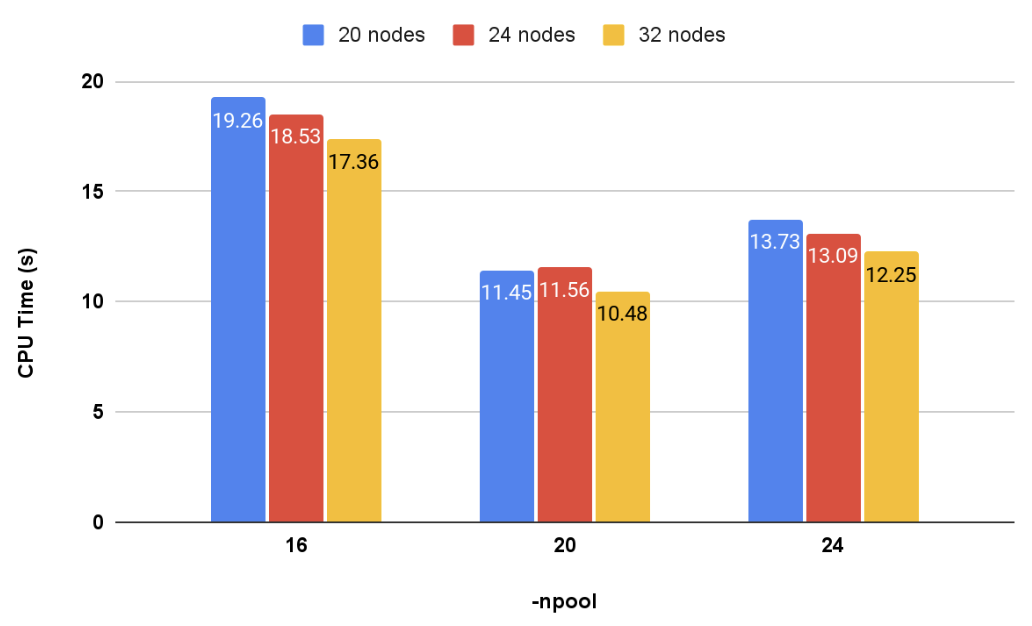
\includegraphics[width=.75\linewidth, height=130pt]{npool}
    \end{figure}

\end{frame}

\subsection{Single Node}

\begin{frame}
	\frametitle{Single Node Performance of Gadi module}
	\framesubtitle{Average of 5 Times}
    \begin{table}
        \centering
        \begin{tabular}{cccl}
           \# CPUs (\texttt{np})  & \# pools (\texttt{npool}) & \makecell{\# linear algebra\\ groups (\texttt{ndiag})} & CPU time [s] \\
            \hline
            48 & 24 & 4 & 1m53.138s \\
            48 & 24 & 1 & 1m53.540s \\
            40 & 20 & 4 & 1m52.794s \\
            40 & 20 & 1 & 1m52.941s \\
        \end{tabular}
        \label{tab:qe-single-module}
    \end{table}
\end{frame}

\begin{frame}
	\frametitle{Single Node Performance of Intel Compiler + Intel MPI}
	\framesubtitle{Average of 5 Times}
    \begin{table}
        \centering
        \begin{tabular}{cccl}
           \# CPUs (\texttt{np})  & \# pools (\texttt{npool}) & \makecell{\# linear algebra\\ groups (\texttt{ndiag})} & CPU time [s] \\
            \hline
            48 & 24 & 4 & 1min58.916s\\
            48 & 24 & 1 & 1min59.004s\\
            40 & 20 & 4 & 1min56.944s\\
            40 & 20 & 1 & 1min57.084s\\
        \end{tabular}
        \label{tab:qe-single-intel}
    \end{table}
\end{frame}

\begin{frame}[fragile]
    \frametitle{Summary}
    \begin{exampleblock}{Script}
        \begin{lstlisting}
#!/bin/bash
#PBS -l walltime=00:10:00
#PBS -l ncpus=40
#PBS -l mem=190GB
#PBS -l software=qe
#PBS -l wd
#PBS -P jx00
#PBS -N QE-single

module load qe
export OMP_NUM_THREADS=1
mpirun -np 40 pw.x -npool 20 -ndiag 4 -inp CeO2.in
        \end{lstlisting}
    \end{exampleblock}
\end{frame}

\begin{frame}[fragile]
    \frametitle{Summary (cont.)}
    
    \begin{alertblock}{Result}
        \begin{figure}
            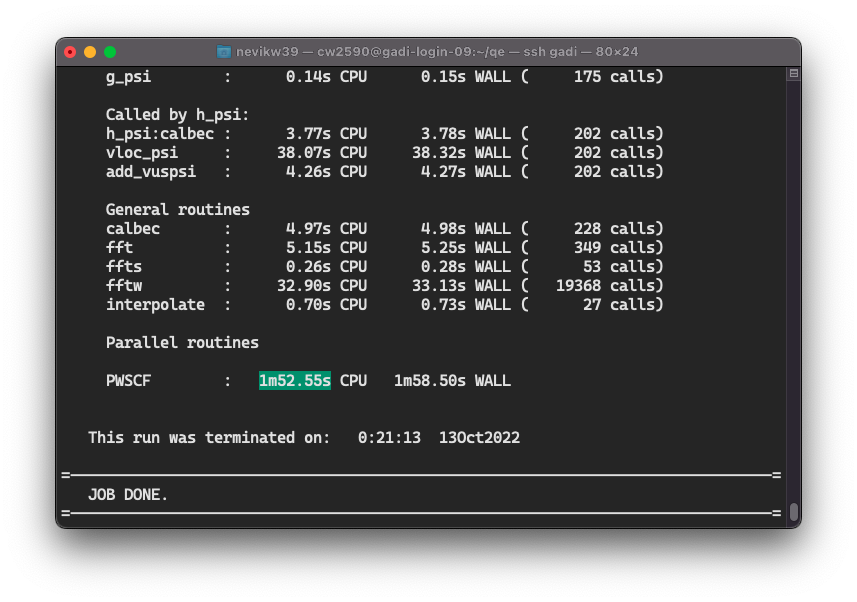
\includegraphics[width=.75\linewidth]{qe-single}
        \end{figure}
    \end{alertblock}
\end{frame}

\subsection{Multiple Nodes}

\begin{frame}
	\frametitle{CPU Time vs. \# Processes}
	\framesubtitle{\texttt{npool}s were 20, 20, 20, 24 resp.; \texttt{ndiag}s were left as default\\The More -np $\centernot\implies$ The Better!!}
    \begin{tikzpicture}
    
    \begin{axis}[
        xlabel=\# Processes,
        xmin=900, xmax=1600,
        ylabel={CPU Time [s]},
        ymin=10, ymax=13.5,
        width=.875\linewidth,
        height=.575\linewidth,
        enlargelimits=0.05,
    ]
    \addplot[smooth, color=nthu, mark=o, nodes near coords={
            $(\pgfmathprintnumber{\pgfkeysvalueof{/data point/x}},
              \pgfmathprintnumber{\pgfkeysvalueof{/data point/y}})$
    }]
    coordinates {
        (960,11.87)(1200,10.45)(1440,12.67)(1536,12.37)
    };
    \end{axis}
    
    \end{tikzpicture}
\end{frame}

\begin{frame}
	\frametitle{\# Iterations vs. \# CPU cores}
    \begin{tikzpicture}
    
    \begin{axis}[
        xlabel=\# CPU cores,
        xmin=900, xmax=1600,
        ylabel=\# Iterations,
        ymin=15, ymax=30,
        width=.875\linewidth,
        height=.625\linewidth,
        enlargelimits=0.05,
    ]
    \addplot[smooth, color=nthu, mark=o, nodes near coords={
            $(\pgfmathprintnumber{\pgfkeysvalueof{/data point/x}},
              \pgfmathprintnumber{\pgfkeysvalueof{/data point/y}})$
    }]
    coordinates {
        (960,24)(1200,20)(1440,24)(1536,26)
    };
    \end{axis}
    
    \end{tikzpicture}
\end{frame}

\begin{frame}
	\frametitle{CPU time vs. \texttt{ndiag} of different CPU cores}
	\framesubtitle{Average of 5 Times}
    \begin{tikzpicture}
    
    \begin{axis}[
        xlabel=$\sqrt{\mathtt{ndiag}}$,
        xmin=0, xmax=85,
        ylabel={CPU time [s]},
        width=\linewidth,
        height=.625\linewidth,
        enlargelimits=0.05,
        legend pos=south east
    ]
    \addplot[smooth, secondary, mark=asterisk] table [col sep=comma] {ndiag_960.csv};
    \addplot[smooth, nthu, mark=Mercedes star] table [col sep=comma] {ndiag_1200.csv};
    \addplot[smooth, accent, mark=diamond] table [col sep=comma] {ndiag_1440.csv};
    \legend{960 cores, 1200 cores, 1440 cores}
    \end{axis}
    
    \end{tikzpicture}
\end{frame}

\begin{frame}
	\frametitle{CPU time vs. \texttt{ndiag} of 1200 CPU cores}
	\framesubtitle{A closer, deeper insight}
    \begin{tikzpicture}
    
    \begin{axis}[
        xlabel=$\sqrt{\mathtt{ndiag}}$,
        xmin=1.5, xmax=6.5,
        xtick distance=1,
        ylabel={CPU time [s]},
        ymin=9.95, ymax=10.125,
        width=\linewidth,
        height=.625\linewidth,
        enlargelimits=0.05,
        legend pos=south east
    ]
    \addplot[smooth, color=nthu, mark=x]
    coordinates {
        (2,10.12176471)(3,9.980645161)(4,9.971612903)(5,10.05529412)(6,10.06333333)
    };
    \end{axis}
    
    \end{tikzpicture}
\end{frame}

\begin{frame}[fragile]
    \frametitle{Conclusion}
    \begin{exampleblock}{Script}
        \begin{lstlisting}
#!/bin/bash
#PBS -l walltime=00:10:00
#PBS -l ncpus=1200
#PBS -l mem=760GB
#PBS -l software=qe
#PBS -l wd
#PBS -P jx00
#PBS -N QE-multi

module load qe
export OMP_NUM_THREADS=1
mpirun -np 1200 pw.x -npool 20 -ndiag 16 -inp CeO2.in
        \end{lstlisting}
    \end{exampleblock}
\end{frame}

\begin{frame}[fragile]
    \frametitle{Conclusion (cont.)}
    \begin{alertblock}{Result}
        \begin{figure}
            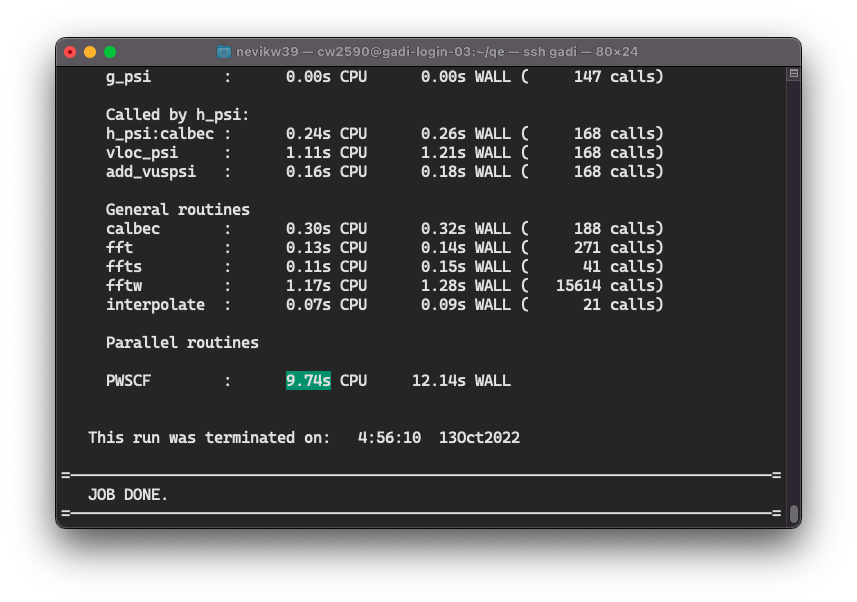
\includegraphics[width=.75\linewidth]{qe-multi}
        \end{figure}
    \end{alertblock}
\end{frame}

\subsection{Additional Supplement}

\begin{frame}
    \frametitle{Additional Supplement}
    \framesubtitle{Compare to QE compiled by ourselves}
        \begin{itemize}
            \item QE compiled by Intel Compiler with IntelMPI will have the better performance when -np equals to 960 instead of 1200 like the QE module on Gadi
        \end{itemize}
        \begin{figure}
            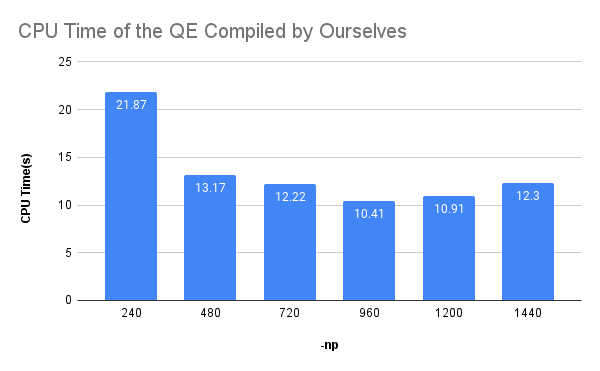
\includegraphics[width=.75\linewidth]{QEaddition.png}
        \end{figure}

\end{frame}

\section{Communications Performance with \texttt{UCX}}

\subsection{Introduction}

\begin{frame}
    \frametitle{Problem}
    \note{\texttt{aftermath}\par Our task is Communications Performance with UCX. The task is about running some python code, these codes creates a central server to synchronize workers, and each worker merges its left and right dataframe. That means the workers need communicate with each others. And our job is to improving performance for this heavy-communication work.

The given benchmark ran on 16 GPUs, on each of which is a worker there with left and right dataframe distributed throughout all GPUs.}
    
    The benchmark is running on 16 GPUs, on each of which is a worker there with left and right dataframe distributed throughout all GPUs.
    
    It is our task that each worker merges its left and right dataframe, which means that a worker need communicate with others at scale.
\end{frame}

\begin{frame}
    \frametitle{Objectives}
    \note{\texttt{nevikw39}\par There are two major metrics to measure the performance of the benchmark we run. We tried to discover the instinct meaning of the two by means of investigating and interpreting the codes provided.\par The first one is the average bandwidth of all workers. For a particular worker, its bandwidth is the average of its left and right dataframe. For each side, it is the summation of size of dataframe transferred from and to all other workers divided by wall time.\par Another one is throughput, which is the number of chunks time the total data processed by all workers divided by wall time.\par We believe that there must be some relation between the two yet that throughput is more comprehensive, so we put more emphasis on it.
}
    
    \begin{block}{Bandwidth of a worker}
        W.L.O.G., let's consider the worker with rank 0.
        
        Define that $\mathsf{bw}=\frac{\sum_{i=1}^{15}size\ of\ \mathsf{Dataframe\ transferred}_i}{\sum_{i=1}^{15}\mathsf{Wall\ time}_i}$.
        
        $$\mathsf{Bandwidth}=\frac{\mathsf{bw}_{left}+\mathsf{bw}_{right}}{2}$$
    \end{block}
    
    \begin{alertblock}{Throughput}
        $$\mathsf{Throughput}=\frac{\mathsf{\#\ chunks}\times\mathsf{Data\ processed}}{\mathsf{Wall\ time}}$$ 
    \end{alertblock}
\end{frame}

\subsection{Optimized Configurations}

\begin{frame}
    \frametitle{Baseline}
    \note{\texttt{aftermath}\par First, we run the job without modifying any code and configuration options, as our baseline. Here, the baseline ran on 16 GPUs over 4 Gadi Volta nodes, for 10 iterations, and for small data set, which means each chunk contains 10 to the power of 6 rows.\par For the baseline, we got the bandwidth 507.21 megabytes per second, and the throughput 4.27 gigabyte per second.}
    
    Average of 10 iterations, small data set (i.e., each chunk with $10^6$ rows), running on 16 GPUs over 4 Gadi Volta nodes.
    
    \begin{block}{Bandwidth}
        \begin{itemize}
            \item 507.21 MiB/s
        \end{itemize}
    \end{block}
    
    \begin{alertblock}{Throughput}
        \begin{itemize}
            \item 4.27 GiB/s
        \end{itemize}
    \end{alertblock}
\end{frame}

\begin{frame}[fragile]
    \frametitle{Enable Hardware Tag Matching}
    \framesubtitle{Avg. of 10 iterations, small data set, Gadi Volta nodes}
    \note{\texttt{nevikw39}\par We managed to find several UCX options that might help. The first option is to enable the hardware tag matching for both \textit{Reliable Connected (RC)} and \textit{Dynamically Connected (DC)} so that these works are offload to NICs.\par We can see that bandwidth somewhat dropped a bit while the throughput increased by a bit. The effect of this option is not so obvious.}
    
    \begin{exampleblock}{Config}
        \begin{lstlisting}
export UCX_RC_MLX5_TM_ENABLE=y
export UCX_DC_MLX5_TM_ENABLE=y
        \end{lstlisting}
    \end{exampleblock}
    
    \begin{block}{Bandwidth}
        \begin{itemize}
            \item 521.87 MiB/s
            \item 102.8\% speedup
        \end{itemize}
    \end{block}
    
    \begin{alertblock}{Throughput}
        \begin{itemize}
            \item 4.36 GiB/s
            \item 102.1\% speedup
        \end{itemize}
    \end{alertblock}
\end{frame}

\begin{frame}[fragile]
    \frametitle{Enable various optimizations intended for homogeneous environment}
    \framesubtitle{Avg. of 10 iterations, small data set, Gadi Volta nodes}
    \note{\texttt{nevikw39}\par Another option we tried is enabling the unified mode, implying that the local transport resources/devices of all entities which connect to each other are the same.\par Nevertheless, this option would be conflict to the \textit{rendezvous} scheme we would choose.\par Similarly, the effect is also not so apparent.}
    
    \begin{exampleblock}{Config}
        \begin{lstlisting}
export UCX_UNIFIED_MODE=y
        \end{lstlisting}
    \end{exampleblock}
    
    \begin{block}{Bandwidth}
        \begin{itemize}
            \item 511.68 MiB/s
            \item 100.8\% speedup
        \end{itemize}
    \end{block}
    
    \begin{alertblock}{Throughput}
        \begin{itemize}
            \item 4.39 GiB/s
            \item 102.8\% speedup
        \end{itemize}
    \end{alertblock}
\end{frame}

\begin{frame}[fragile]
    \frametitle{Increase the amount of buffers added every time the receive / send memory pool grows}
    \framesubtitle{Avg. of 10 iterations, small data set, Gadi Volta nodes}
    \note{\texttt{aftermath}\par The two options here determine how much buffers are added every time the memory pool grows. The above one determines for the receive memory pool, while the below one determines for the send memory pool.

    \par We have thought about that increasing the buffer grow rate may bring better performance for us. Therefore, we’ve tried to double the buffer grow rate. The default value of these two options are both 8, and we’ve modified both of them to 16. After the modification, the bandwidth increases to 513.73 MiB/s, and the throughput increases to 4.68 GiB/s, which really improves the performance.
    
    \par Nonetheless, we found that this option would hardly give rise to ideal promotion in combination with others later.}
    
    \begin{exampleblock}{Config}
        \begin{lstlisting}
export UCX_TCP_RX_BUFS_GROW=16
export UCX_TCP_TX_BUFS_GROW=16
        \end{lstlisting}
    \end{exampleblock}
    
    \begin{block}{Bandwidth}
        \begin{itemize}
            \item 513.73 MiB/s
            \item 101.2\% speedup
        \end{itemize}
    \end{block}
    
    \begin{alertblock}{Throughput}
        \begin{itemize}
            \item 4.68 GiB/s
            \item 109.6\% speedup
        \end{itemize}
    \end{alertblock}
\end{frame}

\begin{frame}[fragile]
    \frametitle{Use \textbf{mutex} instead of \textbf{spinlock} for multithreading support in \texttt{UCP}}
    \framesubtitle{Avg. of 10 iterations, small data set, Gadi Volta nodes}
    \note{\texttt{aftermath}\par For this option, it determines which mechanism to use for Multithreading Support. It is set to n by default, which means not using mutex for multithreading support and using spinlock instead.\par Both spinlock and mutex are common synchronization mechanism.The major difference between them is that the mechanism that mutex uses is sleep-waiting, while spinlock uses busy-waiting.\par There are some pros and cons for both of them, and we have no idea which one is more efficient for the task. Hence we’ve tried both of them and discover that setting this option to y, which means using mutex do improve the performance. The bandwidth comes to 509.99 MiB/s, while the throughput comes to 4.71 GiB/s.}
    
    \begin{exampleblock}{Config}
        \begin{lstlisting}
export UCX_USE_MT_MUTEX=y
        \end{lstlisting}
    \end{exampleblock}
    
    \begin{block}{Bandwidth}
        \begin{itemize}
            \item 509.99 MiB/s
            \item 100.5\% speedup
        \end{itemize}
    \end{block}
    
    \begin{alertblock}{Throughput}
        \begin{itemize}
            \item 4.71 GiB/s
            \item 110.3\% speedup
        \end{itemize}
    \end{alertblock}
\end{frame}

\begin{frame}[fragile]
    \frametitle{Enable \texttt{UCX-Py} non-blocking mode}
    \framesubtitle{Avg. of 10 iterations, small data set, Gadi Volta nodes}
    \note{\texttt{nevikw39}\par In addition, we enabled non-blocking progress mode of UCX-Py. This time, both bandwidth and throughput are about 1.16 times the baseline.}
    
    \begin{exampleblock}{Config}
        \begin{lstlisting}
export UCXPY_NON_BLOCKING_MODE=1
        \end{lstlisting}
    \end{exampleblock}
    
    \begin{block}{Bandwidth}
        \begin{itemize}
            \item 590.62 MiB/s
            \item 116.4\% speedup
        \end{itemize}
    \end{block}
    
    \begin{alertblock}{Throughput}
        \begin{itemize}
            \item 4.96 GiB/s
            \item 116.1\% speedup
        \end{itemize}
    \end{alertblock}
\end{frame}

\begin{frame}[fragile]
    \frametitle{Set \textit{Rendezvous} protocol to use \textit{Active Messages} scheme}
    \framesubtitle{Avg. of 10 iterations, small data set, Gadi Volta nodes}
    \note{\texttt{nevikw39}\par Even though this option is not documented in detail, we tried all available scheme, such as get/put zero copy, pipelined get/put zero copy, ..., finding that only active message brought a significant 30\%-improvement in throughput.}
    
    \begin{exampleblock}{Config}
        \begin{lstlisting}
export UCX_RNDV_SCHEME=am
        \end{lstlisting}
    \end{exampleblock}
    
    \begin{block}{Bandwidth}
        \begin{itemize}
            \item 546.51 MiB/s
            \item 107.7\% speedup
        \end{itemize}
    \end{block}
    
    \begin{alertblock}{Throughput}
        \begin{itemize}
            \item 5.54 GiB/s
            \item 129.7\% speedup
        \end{itemize}
    \end{alertblock}
\end{frame}

\begin{frame}
    \frametitle{Miscellanies}
    \note{\texttt{nevikw39}\par Here are some options we used to try but find no concrete conclusion, such as explicitly use GPU Direct RDMA for HCA to access GPU pages directly, reduce the threshold to switch to RNDV protocol, enlarge copy-out buffer for TCP sending and receiving.}
    
    \begin{itemize}
        \ttfamily
        \item UCX\_IB\_GPU\_DIRECT\_RDMA
        \item UCX\_RNDV\_THRESH
        \item UCX\_TCP\_TX\_SEG\_SIZE\textsf{, }UCX\_TCP\_RX\_SEG\_SIZE
    \end{itemize}
\end{frame}

\subsection{Conclusion}

\begin{frame}[fragile]
    \frametitle{Optimal Combination of Configurations}
    \note{\texttt{aftermath}\par With the above attempts, we combine all configurations that would provide improvement to overall performance. The options we choose are listed here.}
    
    \begin{exampleblock}{Config}
        \begin{lstlisting}
export UCX_RC_TM_ENABLE=y
export UCX_DC_TM_ENABLE=y

export UCX_USE_MT_MUTEX=y

export UCXPY_NON_BLOCKING_MODE=1

export UCX_RNDV_SCHEME=am

export UCX_IB_GPU_DIRECT_RDMA=y
export UCX_RNDV_THRESH=1024
export UCX_TCP_TX_SEG_SIZE=64k
export UCX_TCP_RX_SEG_SIZE=512k
        \end{lstlisting}
    \end{exampleblock}
\end{frame}

\begin{frame}
    \frametitle{Overall Bandwidth Result}
    \framesubtitle{Avg. of 100 iterations on 16 GPUs over 4 Gadi Volta nodes}
    \note{\texttt{aftermath}\par This is our overall bandwidth result. For the small data set, the bandwidth of optimized our config is 1.06 GiB/s, which is more than twice of the baseline. And for the large data set, the bandwidth comes to 1.15 GiB/s, which is almost three times of the baseline.}
    
    \begin{description}
        \item[Small Data Set] 1.06 GiB/s,\\214.0\% speedup in comparison to baseline (507.21 MiB/s)
        \item[Large Data Set] 1.15 GiB/s,\\290.1\% speedup in comparison to baseline (405.89 MiB/s)
    \end{description}
\end{frame}

\begin{frame}
    \frametitle{Overall Throughput Result}
    \framesubtitle{Avg. of 100 iterations on 16 GPUs over 4 Gadi Volta nodes}
    \note{\texttt{nevikw39}\par For the small data set, the throughput of optimized our config is more than twice the one of baseline. And for the large one, it’s almost three times. Note that the speedup of throughput for both data set is not far from the speedup of bandwidth.}
    
    \begin{description}
        \item[Small Data Set] 9.28 GiB/s,\\217.3\% speedup in comparison to baseline (4.27 GiB/s)
        \item[Large Data Set] 12.37 GiB/s,\\281.1\% speedup in comparison to baseline (4.40 GiB/s)
    \end{description}
\end{frame}

\begin{frame}
    \frametitle{Bar graph of throughput speedup}
    \framesubtitle{Avg. of 10 iterations, small data set, Gadi Volta nodes}
    \note{\texttt{nevikw39}\par }
    \note<1>{This is the baseline.}
    \note<2>{These are the speedup of a single option resp.}
    \note<3>{As we can easily find, the optimized combination of configs give rise to as significant improvement of throughput.}
    
    \begin{tikzpicture}
        \centering
        \begin{axis}[
            width=\linewidth,
            height=.625\linewidth,
            ybar,
            bar shift=0,
            symbolic x coords={Base, TM, Uni, BG, mutex, N-B, RNDV, Optimal},
            xmin=Base, xmax=Optimal,
            enlargelimits=true,
        ]
            \addplot[fill=secondary] coordinates {(Base, 1)};
            \only<2->{
                \addplot[fill=nthu] coordinates {
                    (TM, 1.021)
                    (Uni, 1.028)
                    (BG, 1.096)
                    (mutex, 1.103)
                    (N-B, 1.161)
                    (RNDV, 1.297)
                };
            }
            \only<3->{ \addplot[fill=accent] coordinates {(Optimal, 2.173)}; }
        \end{axis}
    \end{tikzpicture}
\end{frame}

\subsection{Running on DGX-A100}

\begin{frame}
    
    \frametitle{Overall Throughput Result on DGX-A100 nodes}
    \framesubtitle{Avg. of 100 iterations on 16 GPUs over 2 Gadi DGX-A100 nodes}
    \begin{table}[h!]
    \centering
    \caption{Average throughput of 100 times (With DGX-A100s)}
    \begin{tabular}{c|c|c}
      \textbf{Chunk size} & \textbf{Default} & \textbf{Optimized Configurations}\\
      \hline
      $10^6$ & 16.66 GiB/s & 16.69 GiB/s\\
      $2.5\times10^7$ & 88.29 GiB/s & \makecell{34.89 GiB/s\footnotemark\\89.00 GiB/s\footnotemark}
    \end{tabular}
    \label{tab:a100}
\end{table}
\end{frame}

\section{Deep-Learning-based DNA Sequence fast decoding}

\subsection{Why do we choose this
model?}

\begin{frame}
    \frametitle{More accurate, more
efficiency}
    \begin{figure}
        \centering
        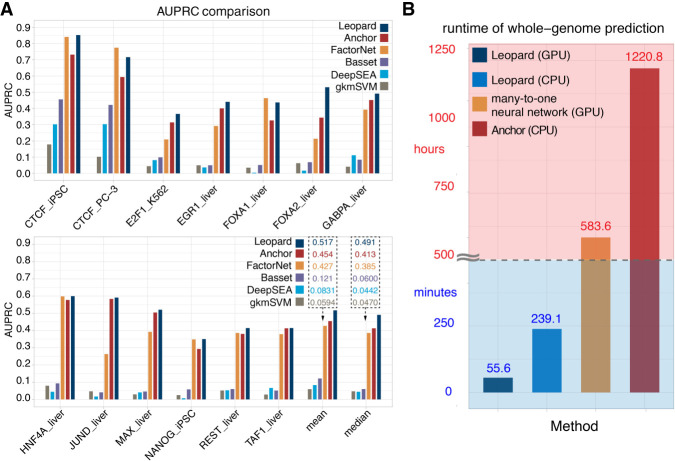
\includegraphics[width=0.78\linewidth]{model_perf}
        \caption{Model performance, adapted from the original paper}
    \end{figure}
\end{frame}

\subsection{Model structure}

\begin{frame}
    \frametitle{Main components}
    \begin{itemize}
        \item Input
        \item Encoder (CCP blocks)
        \item Decoder (UCC blocks)
        \item Output
    \end{itemize}
\end{frame}

\begin{frame}
    \begin{figure}
        \centering
        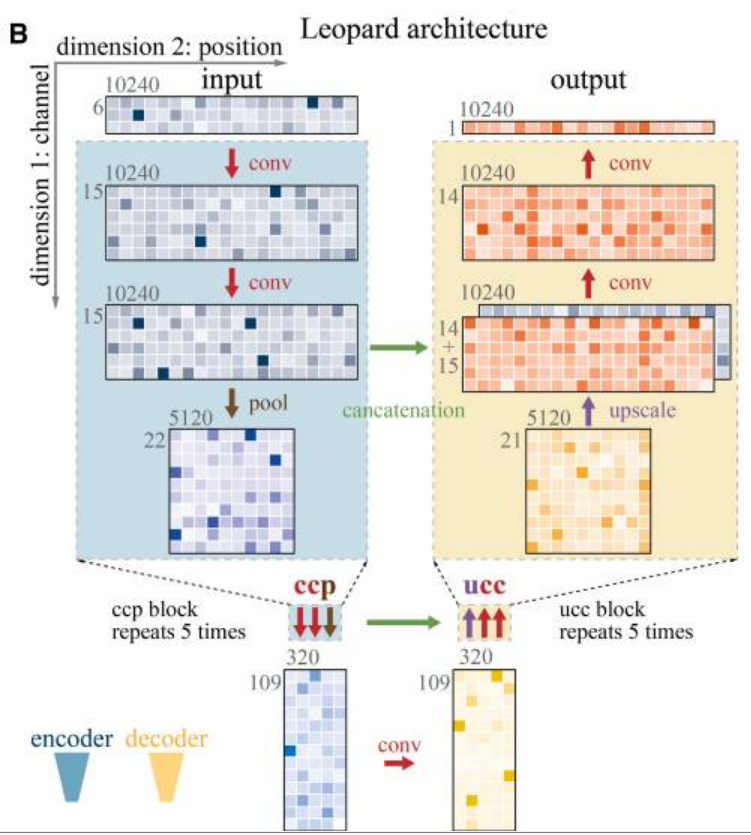
\includegraphics[height=0.87\textheight]{model_struct}
        \caption{Model structure, adapted from the original paper}
    \end{figure}
\end{frame}

\begin{frame}
    \frametitle{Brief summary}
    \framesubtitle{Some facts}
    \begin{itemize}
        \item 61 layers
        \item 475969 parameters 
    \end{itemize}
\end{frame}

\subsection{Tuning}

\subsubsection{Batch size}

\begin{frame}
    \frametitle{Maximum P-R AUC ever reached of various batch sizes}
    \begin{tikzpicture}
    \begin{axis}[
        xlabel=Batch size \textit{(at $\log$ scale)},
        xmode=log,
        ylabel=P-R AUC,
        width=\linewidth,
        height=.625\linewidth,
        enlargelimits=0.05,
        legend pos=south east,
        log ticks with fixed point
    ]
    \addplot[smooth, color=nthu, mark=diamond]
    coordinates {
        (32, 0.5273)(50, 0.523)(64, 0.5297)(80, 0.5264)(100, 0.5041)(500, 0.4729)(800, 0.4505)
    };
    \end{axis}
    \end{tikzpicture}
    
    \note{In our experiments, we follow a hierarchical manner; that is, we first tested \textbf{batch size}, then we adjusted \textbf{learning rate} for a particular \textbf{batch size}.}
\end{frame}

\begin{frame}
    \frametitle{Batch sizes}
    \begin{itemize}
        \item We tried batch size 32, 50, 80 and the default 100, yet their results were not optimal.
    \end{itemize}
\end{frame}

\begin{frame}
    \frametitle{Batch size 64}
    \framesubtitle{Maximum P-R AUC of several learning rates}
    \begin{tikzpicture}
    \begin{axis}[
        xlabel=Learning Rate \textit{(at $\log$ scale)},
        xmode=log,
        ylabel=P-R AUC,
        width=\linewidth,
        height=.625\linewidth,
        enlargelimits=0.05,
        legend pos=south east
    ]
    \addplot[smooth, color=nthu, mark=asterisk]
    coordinates {
        (0.001, 0.4675)(0.0025, 0.5051)(0.005, 0.4985)(0.01, 0.5297)(0.025, 0.4749)(0.05, 0.5024)(0.1, 0.4621)
    };
    \end{axis}
    \end{tikzpicture}

    \note{This is the best \textbf{batch size} we have ever found. We tested
several \textbf{learning rate}, such as \(0.001\), \(0.0025\),
\(0.005\), \(0.01\), \(0.025\), \(0.05\), among of which \(0.01\) gave
rise to optimal result.}
\end{frame}

% \begin{frame}
%     \frametitle{Batch size 100}
%     \begin{itemize}
%         \item The default value
%         \item Better than baseline a bit
%     \end{itemize}
% \end{frame}

\begin{frame}
    \frametitle{Batch size 500}
    \framesubtitle{Overfitting}
    \begin{tikzpicture}
    
    \begin{axis}[
        xlabel=Epoch,
        ylabel=P-R AUC,
        width=\linewidth,
        height=.625\linewidth,
        enlargelimits=0.05,
        legend pos=south east
    ]
    \addplot[smooth, secondary] table [col sep=comma] {train.csv};
    \addplot[smooth, accent] table [col sep=comma] {valid.csv};
    \legend{Training, Validation}
    \end{axis}
    
    \end{tikzpicture}
    
    \note{We encounter severe \emph{\textbf{overfitting}} when it comes to this \textbf{batch size}; that is, \emph{P-R AUC} could increase up to about \(0.96\) for the training set, whereas the ones for validation set were as low as \(0.25\). What's worse, since we increased the patience of early stop to 10, it exhausted the 2-hour wall time.}
\end{frame}

\begin{frame}
    \frametitle{Batch size 800}
    \framesubtitle{Validation loss cannot converge to less than $10^{-3}$ (Note that y-axis is at $\log$ scale)}
    \begin{tikzpicture}
    
    \begin{axis}[
        xlabel=Epoch,
        xmin=3,
        ylabel=Validation Loss \textit{(at $\log$ scale)},
        ymode=log,
        width=\linewidth,
        height=.625\linewidth,
        enlargelimits=0.05,
        legend pos=north east
    ]
    \addplot[smooth, accent] table [col sep=comma] {loss_800.csv};
    \addplot[smooth, nthu] table [col sep=comma] {loss_100.csv};
    \addplot[smooth, secondary] table [col sep=comma] {loss_64.csv};
    \legend{Batch size 800, Batch size 100, Batch size 64}
    \end{axis}
    
    \end{tikzpicture}
    
    \note{The maximum \textbf{batch size} for V100 is 800 since it consumes about 31GB GPU memory. For this \textbf{batch size}, the converge rate of validation loss were quite slow despite of \textbf{learning rate}. As a consequence, the results were also not so good.}
\end{frame}

\begin{frame}
    \frametitle{Batch size 1600, 2000, 2500}
    \begin{itemize}
        \item On A100 only since memory usage would be over about 31GiB!
        \item Loss could hardly converge, similar with batch size 800
    \end{itemize}
\end{frame}

\begin{frame}
    \frametitle{Parallelization via Multiple
GPUs}
    \framesubtitle{Performance always counts more!}
    \begin{tikzpicture}
    \begin{axis}[
        xlabel=\# GPU,
        xmin=0.5, xmax=4.5,
        xtick distance=1,
        ylabel=P-R AUC,
        width=\linewidth,
        height=.625\linewidth,
        enlargelimits=0.05,
        legend pos=south east
    ]
    \addplot[smooth, color=nthu, mark=Mercedes star]
    coordinates {
        (1, 0.5297)(2, 0.4815)(3, 0.4461)(4, 0.4780)
    };
    \end{axis}
    \end{tikzpicture}
    
    \note{We also managed to parallelize the training and utilized multiple GPUs. Nonetheless, the performance would decline a lot. Furthermore, the metrics would drop suddenly and dramatically after the number of GPU was over a value. We guessed that it might due to the simple, linear scale of \textbf{learning rate}, trying to find ad-hoc optimal \textbf{learning rate} for different number of GPU yet in vain.\par Eventually, we decide to train on only a single GPU since we believe that the performance counts more. Still, we provide the job script to train across two A100s.}
\end{frame}

\begin{frame}
    \frametitle{Volta and Amp\`{e}re GPUs}
    % NVIDIA Volta V100 vs. NVIDIA Amp\`{e}re A100
    \begin{itemize}
        \item NVIDIA Volta V100: Main GPUs on Gadi
        \item NVIDIA Amp\`{e}re A100: Faster and more memory
    \end{itemize}
\end{frame}

\subsection{Result}

\begin{frame}
    \frametitle{Hyperparameters and environments}
    \begin{description}
        \item[Batch Size] 64
        \item[Learning Rate] 0.01
        \item[\# GPU] 1
    \end{description}
\end{frame}

\begin{frame}

\begin{longtable}[]{@{}
  >{\centering\arraybackslash}p{(\columnwidth - 10\tabcolsep) * \real{0.0775}}
  >{\centering\arraybackslash}p{(\columnwidth - 10\tabcolsep) * \real{0.2326}}
  >{\centering\arraybackslash}p{(\columnwidth - 10\tabcolsep) * \real{0.1628}}
  >{\centering\arraybackslash}p{(\columnwidth - 10\tabcolsep) * \real{0.1395}}
  >{\centering\arraybackslash}p{(\columnwidth - 10\tabcolsep) * \real{0.2326}}
  >{\raggedleft\arraybackslash}p{(\columnwidth - 10\tabcolsep) * \real{0.1550}}@{}}
\caption{Performance of Single GPU}\tabularnewline
\toprule()
\begin{minipage}[b]{\linewidth}\centering
GPU Type
\end{minipage} & \begin{minipage}[b]{\linewidth}\centering
Loss \emph{(Binary Crossentropy)}
\end{minipage} & \begin{minipage}[b]{\linewidth}\centering
~P-R AUC~
\end{minipage} & \begin{minipage}[b]{\linewidth}\centering
Dice coeff.
\end{minipage} & \begin{minipage}[b]{\linewidth}\centering\small
Binary Int. of Union
\end{minipage} & \begin{minipage}[b]{\linewidth}\raggedleft
Training Time {[}s{]}
\end{minipage} \\
\midrule()
\endfirsthead
\toprule()
\begin{minipage}[b]{\linewidth}\centering
GPU Type
\end{minipage} & \begin{minipage}[b]{\linewidth}\centering
Loss \emph{(Binary Crossentropy)}
\end{minipage} & \begin{minipage}[b]{\linewidth}\centering
~P-R AUC~
\end{minipage} & \begin{minipage}[b]{\linewidth}\centering
Dice coefficient
\end{minipage} & \begin{minipage}[b]{\linewidth}\centering
Binary Intersection of Union
\end{minipage} & \begin{minipage}[b]{\linewidth}\raggedleft
Training Time {[}s{]}
\end{minipage} \\
\midrule()
\endhead
V100 & \(7.2768\times10^{-4}\) & \(0.5297\) & \(0.3705\) & \(0.3625\) &
\(3170.19\) \\
A100 & \(7.3153\times10^{-4}\) & \(0.5288\) & \(0.4109\) & \(0.3701\) &
\(941.63\) \\
\bottomrule()
\end{longtable}

\end{frame}

% \begin{frame}{Leopard Unet Model}
%     \begin{description}
%         \item[loss] = 0.000778545334469527
%         \item[pr auc] = 0.5140474438667297
%         \item[dice coef] = 0.4189634919166565
%         \item[binary io u] = 0.3518095314502716
%         \item[training time] = 2021.0820441246033
%     \end{description}
% \end{frame}

% \begin{frame}{CNN}
%     \begin{description}
%         \item[loss] : 0.0008428519358858466
%         \item[pr auc] : 0.4610700011253357
%         \item[dice coef] : 0.34029775857925415
%         \item[binary io u] : 0.311911940574646
%         \item[training time] : 2006.29443693161
%     \end{description}
% \end{frame}

\end{document}